\def\mytitle{DIGITAL COMMUNICATIONS}
\def\myauthor{V.GOKULKUMAR}
\def\contact{velicharla@outlook.com}
\def\mymodule{Future Wireless Communication (FWC)}
\documentclass[10pt, a4paper]{article}
\usepackage[a4paper,outer=1.5cm,inner=1.5cm,top=1.75cm,bottom=1.5cm]{geometry}
\twocolumn
\usepackage{gauss}
\usepackage{graphicx}
\graphicspath{{./images/}}
\usepackage[colorlinks,linkcolor={black},citecolor={blue!80!black},urlcolor={blue!80!black}]{hyperref}
\usepackage[parfill]{parskip}
\usepackage{lmodern}
\usepackage{tikz}
\usepackage{bm}
%\documentclass[tikz, border=2mm]{standalone}
\usepackage{karnaugh-map}
%\documentclass{article}
\usepackage{tabularx}
\usepackage{circuitikz}
\usetikzlibrary{calc}
\usepackage{enumitem}
\usepackage{amsmath}
\usepackage{bm,amsmath}
\usepackage{amssymb}
\renewcommand*\familydefault{\sfdefault}
\usepackage{watermark}
\usepackage{lipsum}
\usepackage{xcolor}
\usepackage{listings}
\usepackage{float}
\usepackage{titlesec}
       \usepackage[latin1]{inputenc}
       \usepackage{color}
       \usepackage{array}
       \usepackage{longtable}
       \usepackage{calc}
       \usepackage{multirow}
       \usepackage{hhline}
       \usepackage{ifthen}
       
\providecommand{\sbrak}[1]{\ensuremath{{}\left[#1\right]}}
\titlespacing{\subsection}{1pt}{\parskip}{3pt}
\titlespacing{\subsubsection}{0pt}{\parskip}{-\parskip}
\titlespacing{\paragraph}{0pt}{\parskip}{\parskip}
\newcommand{\figuremacro}[5]{
    \begin{figure}[#1]
        \centering
        \includegraphics[width=#5\columnwidth]{#2}
        \caption[#3]{\textbf{#3}#4}
        \label{fig:#2}
    \end{figure}
}
\providecommand{\brak}[1]{\ensuremath{\left(#1\right)}}

\lstset{
frame=single, 
breaklines=true,
columns=fullflexible
}




\thiswatermark{\centering \put(181,-119.0){
\includegraphics[scale=0.13]{iith_logo3}} }
\title{\mytitle}
\author{\myauthor\hspace{1em}\\\contact\\FWC22034\hspace{6.5em}IITH\hspace{0.5em}\mymodule\hspace{6em}ASSIGNMENT}
\begin{document}



\newtheorem{theorem}{Theorem}[section]
\newtheorem{problem}{Problem}
\newtheorem{proposition}{Proposition}[section]
\newtheorem{lemma}{Lemma}[section]
\newtheorem{corollary}[theorem]{Corollary}
\newtheorem{example}{Example}[section]
\newtheorem{definition}[problem]{Definition}
%\newtheorem{thm}{Theorem}[section] 
%\newtheorem{defn}[thm]{Definition}
%\newtheorem{algorithm}{Algorithm}[section]
%\newtheorem{cor}{Corollary}
\newcommand{\BEQA}{\begin{eqnarray}}
\newcommand{\EEQA}{\end{eqnarray}}
\newcommand{\define}{\stackrel{\triangle}{=}}
\bibliographystyle{IEEEtran}
%\bibliographystyle{ieeetr}
\providecommand{\mbf}{\mathbf}
\providecommand{\pr}[1]{\ensuremath{\Pr\left(#1\right)}}
\providecommand{\qfunc}[1]{\ensuremath{Q\left(#1\right)}}
\providecommand{\sbrak}[1]{\ensuremath{{}\left[#1\right]}}
\providecommand{\lsbrak}[1]{\ensuremath{{}\left[#1\right.}}
\providecommand{\rsbrak}[1]{\ensuremath{{}\left.#1\right]}}
\providecommand{\brak}[1]{\ensuremath{\left(#1\right)}}
\providecommand{\lbrak}[1]{\ensuremath{\left(#1\right.}}
\providecommand{\rbrak}[1]{\ensuremath{\left.#1\right)}}
\providecommand{\cbrak}[1]{\ensuremath{\left\{#1\right\}}}
\providecommand{\lcbrak}[1]{\ensuremath{\left\{#1\right.}}
\providecommand{\rcbrak}[1]{\ensuremath{\left.#1\right\}}}
%\theoremstyle{remark}
\newtheorem{rem}{Remark}
\newcommand{\sgn}{\mathop{\mathrm{sgn}}}
%\providecommand{\abs}[1]{\left\vert#1\right\vert}
\providecommand{\res}[1]{\Res\displaylimits_{#1}} 
%\providecommand{\norm}[1]{\left\lVert#1\right\rVert}
%\providecommand{\norm}[1]{\lVert#1\rVert}
\providecommand{\mtx}[1]{\mathbf{#1}}
%\providecommand{\mean}[1]{E\left[ #1 \right]}
\providecommand{\gauss}[2]{\mathcal{N}\ensuremath{\left(#1,#2\right)}}
\providecommand{\fourier}{\overset{\mathcal{F}}{ \rightleftharpoons}}
%\providecommand{\hilbert}{\overset{\mathcal{H}}{ \rightleftharpoons}}
\providecommand{\system}{\overset{\mathcal{H}}{ \longleftrightarrow}}
	%\newcommand{\solution}[2]{\vec{Solution:}{#1}}
\newcommand{\solution}{\noindent \textbf{Solution: }}
\newcommand{\cosec}{\,\text{cosec}\,}
\providecommand{\dec}[2]{\ensuremath{\overset{#1}{\underset{#2}{\gtrless}}}}
\newcommand{\myvec}[1]{\ensuremath{\begin{pmatrix}#1\end{pmatrix}}}
\newcommand{\mydet}[1]{\ensuremath{\begin{vmatrix}#1\end{vmatrix}}}
%\numberwithin{equation}{section}
%\numberwithin{equation}{subsection}
%\numberwithin{problem}{section}
%\numberwithin{definition}{section}
\makeatletter
\@addtoreset{figure}{problem}
\makeatother
\let\StandardTheFigure\thefigure
\let\vec\mathbf
%\renewcommand{\thefigure}{\theproblem.\arabic{figure}}
%\renewcommand{\thefigure}{\theproblem}
%\setlist[enumerate,1]{before=\renewcommand\theequation{\theenumi.\arabic{equation}}
%\counterwithin{equation}{enumi}

	\maketitle
	\section{Random numbers}
 \subsection{Uniform Random Numbers}
Let $U$ be a uniform random variable between 0 and 1.
\begin{enumerate}[label=\thesection.\arabic*
,ref=\thesection.\theenumi]
\item Generate $10^6$ samples of $U$ using a C program and save into a file called uni.dat .

\begin{center}
\fbox{\parbox{8.2cm}{\url{https://github.com/velicharlagokulkumar/digital-communications/blob/main/codes/chapter-5/5.1.1/uni.dat}}}
\end{center}
\item
Load the uni.dat file into python and plot the empirical CDF of $U$ using the samples in uni.dat. The CDF is defined as
\begin{align}
F_{U}(x) = \pr{U \le x}
\end{align}
\\
\solution  The following code plots Fig. \ref{fig:uni_cdf}
\begin{center}
\fbox{\parbox{8.2cm}{\url{https://github.com/velicharlagokulkumar/digital-communications/blob/main/codes/chapter-5/5.1.2/cdf_plot.py}}}
\end{center}
\begin{figure}[!ht]
\centering
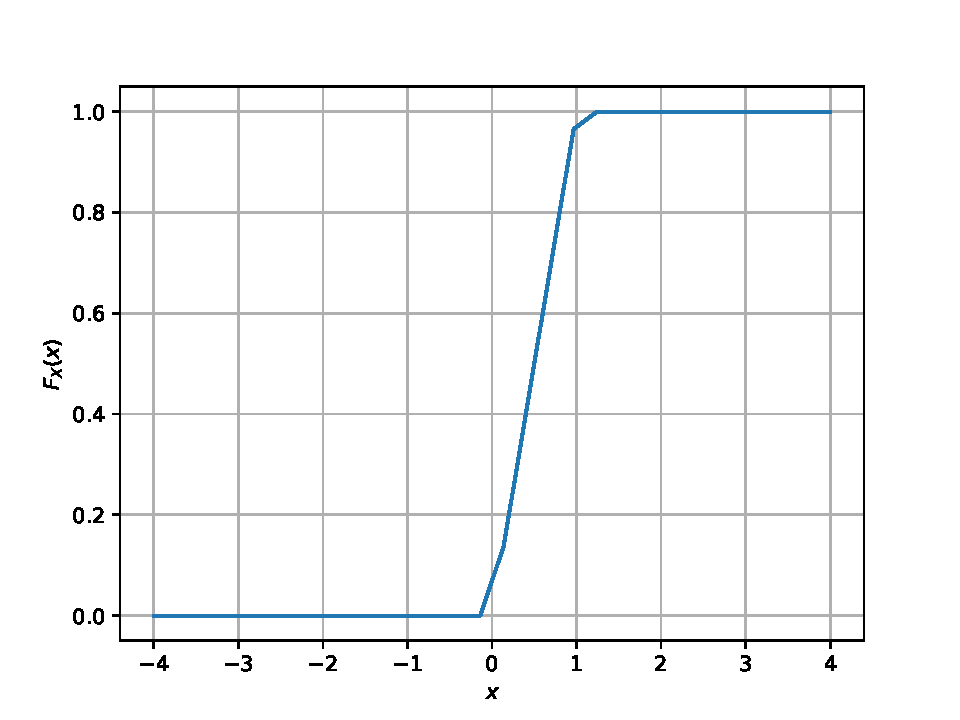
\includegraphics[scale=0.5]{images/uni_cdf.png}
\caption{CDF}
\end{figure}
\item
Find a  theoretical expression for $F_{U}(x)$.
\\
Uniform Random variable:
 $$
\begin{aligned}
& \left.\begin{array}{ll}
f_U(x)=\frac{1}{b-a} & a \leq x \leq b \\
\ \ \ \ \ \ \ \ \ =0 & \text { elsewhere }
\end{array}\right\} \begin{array}{l}
\text { where a and } \\
b \text { are real } \\
\text { constants } \\
-\alpha<a<\alpha \\
\& b>a
\end{array} \\
& F_U(x)=\int_{-\infty}^x f_x(x) d x \\
& =\int_{-\infty}^x \frac{1}{b-a} \cdot d x \\
& =\left.\frac{1}{b-a} \cdot x\right|_a ^x \\
& =\frac{x-a}{b-a} \\
\end{aligned}
$$

$$
F_U(x)=\left\{\begin{array}{lr}
0 & x<a \\
(x-a) /(b-a) & a \leq x<b \\
1 & b \leq x
\end{array}\right.
$$

\item
The mean of $U$ is defined as
%
\begin{equation}
E\sbrak{U} = \frac{1}{N}\sum_{i=1}^{N}U_i
\end{equation}
%
and its variance as
%
\begin{equation}
\text{var}\sbrak{U} = E\sbrak{U- E\sbrak{U}}^2 
\end{equation}
Write a C program to  find the mean and variance of $U$. 


\begin{lstlisting}
#include <stdio.h>
#include <stdlib.h>
#include <math.h>
#include "coeffs.h"

int  main(void) //main function begins
{
 
//Uniform random numbers
uniform("uni.dat", 1000000);

//Mean of uniform
printf("%lf\n",mean("uni.dat"));
//Variance of uniform
printf("%lf",variance("uni.dat"));
return 0;
}
\end{lstlisting}
\begin{lstlisting}
double mean(char *str)
{
int i=0,c;
FILE *fp;
double x, temp=0.0;

fp = fopen(str,"r");
//get numbers from file
while(fscanf(fp,"%lf",&x)!=EOF)
{
//Count numbers in file
i=i+1;
//Add all numbers in file
temp = temp+x;
}
fclose(fp);
temp = temp/(i-1);
return temp;

}
\end{lstlisting}
\begin{lstlisting}
double variance(char *str)
{
int i=0,j=0,c;
FILE *fp;
double x, temp=0.0,value,sumsqr=0,variance=0.0;

fp = fopen(str,"r");
//get numbers from file
while(fscanf(fp,"%lf",&x)!=EOF)
{
//Count numbers in file
i=i+1;
//Add all numbers in file
temp = temp+x;
}
fclose(fp);
temp = temp/(i-1);
fp = fopen(str,"r");
while(fscanf(fp,"%lf",&x)!=EOF)
{
  j=j+1;
  value=x-temp;
     sumsqr=sumsqr+value*value;
}
fclose(fp);
variance = sumsqr/(j-1);
return variance;
}
\end{lstlisting}
Result:
\begin{lstlisting}
  mean=0.500137 
  variance=0.83251
\end{lstlisting}
\begin{center}
\fbox{\parbox{8.2cm}{\url{https://github.com/velicharlagokulkumar/digital-communications/blob/main/codes/chapter-5/5.1.4/uniform.c}}}
\end{center}

\item Verify your result theoretically given that
%
\begin{equation}
E\sbrak{U^k} = \int_{-\infty}^{\infty}x^kdF_{U}(x)
\end{equation}
\begin{align}
Mean:
 \mathrm{E}[U]=\int_a^b x \cdot \frac{1}{b-a} d x=\frac{b^2-a^2}{2} \cdot \frac{1}{b-a} \\ =\frac{(b-a)(b+a)}{2} \cdot \frac{1}{b-a} \\=\frac{b+a}{2} 
 \\ Here \  a=0,b=1
 \\ \mu= \mathrm{E}[X]= \frac{1}{2} = 0.5
\\
 \mathrm{E}[U^2]=\int_a^b x^2 \cdot \frac{1}{b-a} d x=\frac{b^3-a^3}{3} \cdot \frac{1}{b-a} \\ =\frac{a^2+ab+b^2}{3}\\
 Variance:
 \sigma^2=E\left(U^2\right)-[E(U)]^2
 =\frac{(a-b)^2}{12}\\
  \sigma^2=0.834
\end{align}
\end{enumerate}

 \subsection{Central Limit Theorem}
 
\begin{enumerate}

%
\item
Generate $10^6$ samples of the random variable
%
\begin{equation}
X = \sum_{i=1}^{12}U_i -6
\end{equation}
%
using a C program, where $U_i, i = 1,2,\dots, 12$ are  a set of independent uniform random variables between 0 and 1
and save in a file called gau.dat

\begin{center}
\fbox{\parbox{8.2cm}{\url{https://github.com/velicharlagokulkumar/digital-communications/blob/main/codes/chapter-5/5.2.1/gau.dat}}}
\end{center}

\item
Load gau.dat in python and plot the empirical CDF of $X$ using the samples in gau.dat. What properties does a CDF have?
\\
\solution The CDF of $X$ is plotted in Fig.
\begin{center}
\fbox{\parbox{8.2cm}{\url{https://github.com/velicharlagokulkumar/digital-communications/blob/main/codes/chapter-5/5.2.2/cdf_plot.py}}}
\end{center}

\begin{figure}
\centering
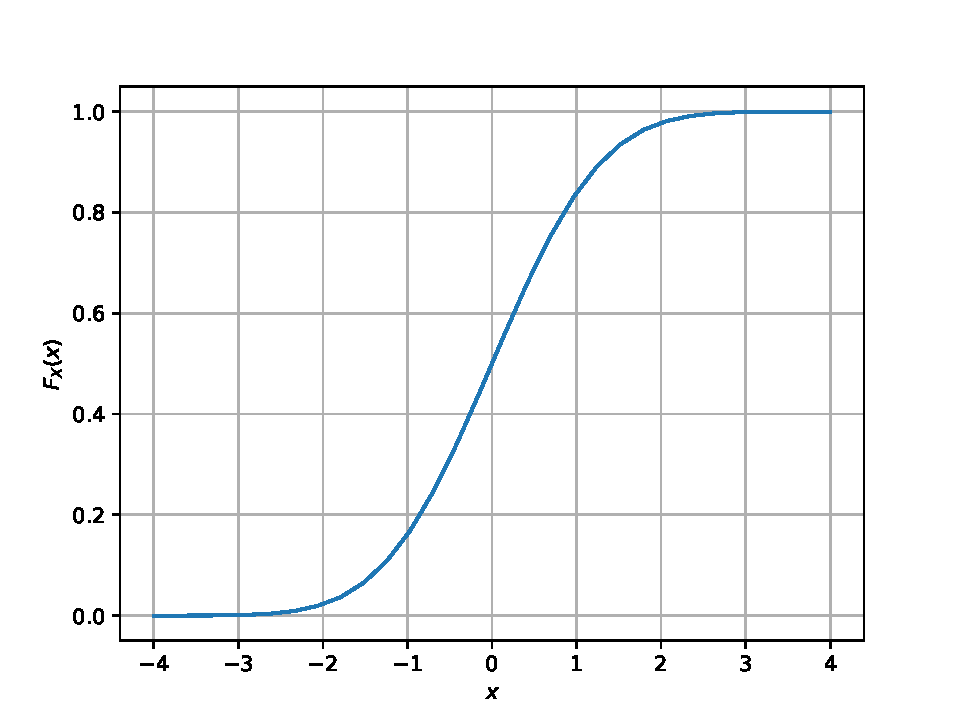
\includegraphics[scale=0.5]{images/gau_cdf.pdf}
\caption{CDF of X}
\label{fig:gauss_cdf}
\end{figure}
\item
Load gau.dat in python and plot the empirical PDF of $X$ using the samples in gau.dat. The PDF of $X$ is defined as
\begin{align}
p_{X}(x) = \frac{d}{dx}F_{X}(x)
\end{align}
What properties does the PDF have?
\\
\solution The PDF of $X$ is plotted in Fig. \ref{fig:gauss_pdf} using the code below
\begin{center}
\fbox{\parbox{8.2cm}{\url{https://github.com/velicharlagokulkumar/digital-communications/blob/main/codes/chapter-5/5.2.3/pdf_plot.py}}}
\end{center}
\begin{figure}
\centering
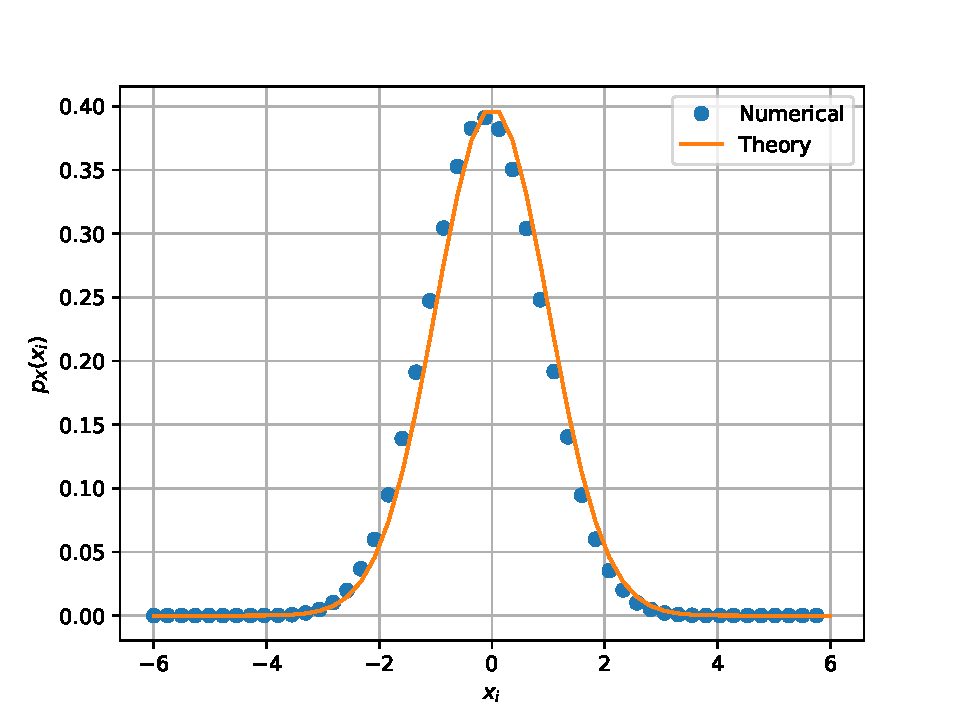
\includegraphics[scale=0.5]{images/gau_pdf.pdf}
\caption{The PDF of $X$}
\label{fig:gauss_pdf}
\end{figure}


 \item Find the mean and variance of $X$ by writing a C program.
\begin{lstlisting}
#include <stdio.h>
#include <stdlib.h>
#include <math.h>
#include "coeffs.h"

int  main(void) //main function begins
{
 
//gaussian random numbers
gaussian("gau.dat", 1000000);

//Mean ,variance of gaussian
printf("%lf\n",mean("gau.dat"));
printf("%lf",variance("gau.dat"));
return 0;
}
\end{lstlisting}
\begin{lstlisting}
  mean=-0.000283
  variance=0.999702
\end{lstlisting}

\begin{center}
\fbox{\parbox{8.2cm}{\url{https://github.com/velicharlagokulkumar/digital-communications/blob/main/codes/chapter-5/5.2.4/gauss.c}}}
\end{center}

\item Given that 
\begin{align}
p_{X}(x) = \frac{1}{\sqrt{2\pi}}\exp\brak{-\frac{x^2}{2}}, -\infty < x < \infty,
\end{align}
repeat the above exercise theoretically.
$$
\begin{aligned}
& E(X)=\frac{1}{\sqrt{2 \pi}} \int_{-\infty}^{\infty} x e^{-\frac{x^2}{2}} d x \\
& =0 \quad \text { ( odd function) } \\
& E\left(X^2\right)=\frac{1}{\sqrt{2 \pi}} \int_{-\infty}^{\infty} x^2 e^{-\frac{x^2}{2}} d x \quad \text { (evenfunction) } \\
& =\frac{2}{\sqrt{2 \pi}} \int_0^{\infty} x^2 e^{-\frac{x^2}{2}} d x \\
& =\frac{2}{\sqrt{2 \pi}} \int_0^{\infty} \sqrt{2 u} e^{-u} d u \quad\left(\text { Let } \frac{x^2}{2}=u\right) \\
& =\frac{2}{\sqrt{\pi}} \int_0^{\infty} e^{-u} u^{\frac{3}{2}-1} d u \\
& =\frac{2}{\sqrt{\pi}} \Gamma\left(\frac{3}{2}\right) \\
& =\frac{1}{\sqrt{\pi}} \Gamma\left(\frac{1}{2}\right) \\
& =1 \\
&
\end{aligned}
$$
where we have used the fact that
$$
\because \Gamma(n)=(n-1) \Gamma(n-1) ; \Gamma\left(\frac{1}{2}\right)=\sqrt{\pi}
$$
Thus, the variance is
$$
\sigma^2=E(X)^2-E^2(X)=1
$$
\end{enumerate}




\subsection{From Uniform to Other}
\begin{enumerate}
\item Generate samples of 
%
\begin{equation}
V = -2\ln\brak{1-U}
\label{eq:probman_V_cdf_sim}
\end{equation}
%
and plot its CDF.
\begin{figure}[!ht]
\centering
\includegraphics[scale=0.5]{images/quantile.png}
\caption{CDF}
\end{figure}
\item Find a theoretical expression for $F_V(x)$.
The CDF of $V$ is defined as 
\begin{align}
    F_V(v) &= pr(V \le v) \\
           &= pr( -2 \ln(1-U)\le v) \\
           &= pr(\ln(1-U) \ge -\frac{v}{2})\\
           &= pr(1-U \ge \exp\brak{-\frac{v}{2}})\\
           &= pr(U \le 1- \exp\brak{-\frac{v}{2}})\\
           &= F_U\brak{1- \exp\brak{-\frac{v}{2}}}
%           &=  (1-(exp(-v/2))
\label{eq:probman_cdf_V_temp}
\end{align}
\begin{align}
F_U(x) = 
\begin{cases}
0 &  x < 0 \\
x & 0 \le x \le 1 \\
1 & x > 1
\end{cases}
\end{align}
%
Substituting the above in \eqref{eq:probman_cdf_V_temp},
%
\begin{multline}
F_U\brak{1- \exp\brak{-\frac{v}{2}}} =
\\
\begin{cases}
0 &  1- \exp\brak{-\frac{v}{2}} < 0 \\
1- \exp\brak{-\frac{v}{2}} & 0 \le 1- \exp\brak{-\frac{v}{2}} \le 1 \\
1 & 1- \exp\brak{-\frac{v}{2}} > 1
\end{cases}
\end{multline}
%
After some algebra, the above conditions yield
\begin{align}
F_V(v) = 
\begin{cases}
0 & v < 0 \\
1- exp\brak{-\frac{v}{2}} & v \ge 0
\end{cases}
\label{eq:probman_V_cdf_anal}
\end{align}
%
which is the CDF of the exponential distribution with parameter $\frac{1}{2}$. 
\end{enumerate}


\subsection{Triangular Distribution}
\begin{enumerate}[label=\thesection.\arabic*
,ref=\thesection.\theenumi]
%
\item Generate 
	\begin{align}
		T = U_1+U_2
	\end{align}
\item Find the CDF of $T$.
\item Find the PDF of $T$.
\item Find the theoretical expressions for the PDF and CDF of $T$.
\item Verify your results through a plot. 
\end{enumerate}







\section{transfromations of R.V}
\subsection{Gaussian to Other}
\begin{enumerate}
\item
Let $X_1 \sim  (0,1) $ and $X_2 \sim (0,1)$. Plot the CDF and PDF of
%
\begin{equation}
V = X_1^2 + X_2^2 
\end{equation}

\begin{center}
\fbox{\parbox{8.2cm}{\url{https://github.com/velicharlagokulkumar/digital-communications/blob/main/codes/chapter-7/7.1.1/7.1.1_CDF.py}}}
\end{center}
\begin{center}
\fbox{\parbox{8.2cm}{\url{https://github.com/velicharlagokulkumar/digital-communications/blob/main/codes/chapter-7/7.1.1/7.1.1_PDF.py}}}
\end{center}


\begin{figure}[!ht]
\centering
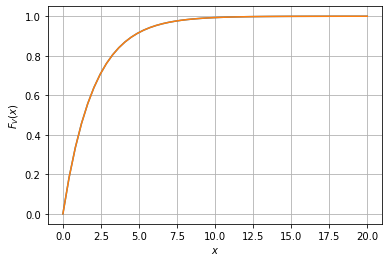
\includegraphics[scale=0.5]{images/6.1.1.cdf.png}
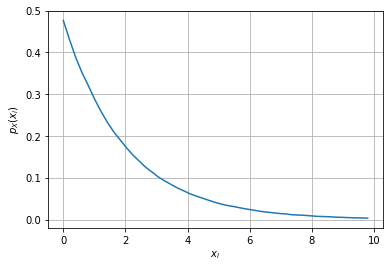
\includegraphics[scale=0.5]{images/6.1.1.pdf.png}
\caption{CDF,PDF of $V$}
\end{figure}

\item
If
%
\begin{equation}
F_{V}(x) = 
\begin{cases}
1 - e^{-\alpha x} & x \geq 0 \\
0 & x < 0,
\end{cases}
\label{eq:probman_F_V_alpha}
\end{equation}
%
find $\alpha$.
\\
For the value $\alpha=0.5$, the theory matches the simulation.  
The following code generates the CDF of $V$ in Fig. 
Fig. 

\begin{figure}[!ht]
\centering
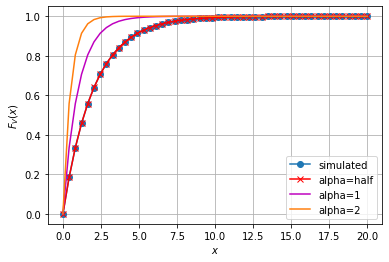
\includegraphics[scale=0.5]{images/6.1.2.png}
\caption{CDF of $V$}
\end{figure}
%
%
\item
\label{ch3_raleigh_sim}
Plot the CDF and PDf of
%
\begin{equation}
A = \sqrt{V}
\end{equation}
%
 The CDF and PDF of A are plotted in Figs. \ref{fig:probman_trans_cdf_A} and \ref{fig:probman_trans_PDf_A}
using the codes below.

\begin{figure}[!ht]
\centering
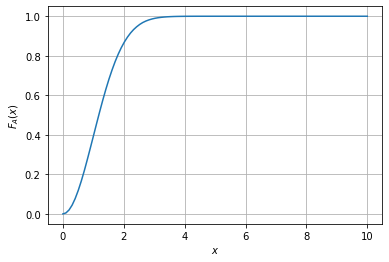
\includegraphics[scale=0.5]{images/6.1.3.cdf.png}
\caption{CDF}
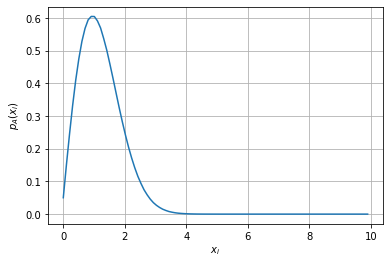
\includegraphics[scale=0.5]{images/6.1.3.pdf.png}
\caption{PDF}
\end{figure}

\end{enumerate}
\begin{center}
\fbox{\parbox{8.2cm}{\url{https://github.com/velicharlagokulkumar/digital-communications/blob/main/codes/chapter-7/7.1.3/7.1.3_CDF.py}}}
\end{center}
\begin{center}
\fbox{\parbox{8.2cm}{\url{https://github.com/velicharlagokulkumar/digital-communications/blob/main/codes/chapter-7/7.1.3/7.1.3_PDF.py}}}
\end{center}

\subsection{Conditional Probability}
\begin{enumerate}
\item
\label{ch4_sim}
Plot 
\begin{equation}
P_e = \pr{\hat{X} = -1|X=1}
\end{equation}
%
for 
\begin{equation}
Y = AX+N,
\end{equation}
where $A$ is Raleigh with $E\sbrak{A^2} = \gamma, N \sim \mathcal{N}(0,1) \in \brak{-1,1}$ for $0 \le \gamma \le 10$ dB.
\\


%
\item
Assuming that $N$ is a constant, find an expression for $P_e$.  Call this $P_e(N)$.
\\
The estimated value $\hat{X}$ is given by
\begin{align}
\hat{X} = 
\begin{cases}
+1 & Y>0\\
-1 & Y<0
\end{cases}
\end{align}
For $X = 1$, 
\begin{align}
Y &= A + N\\
P_e &= \pr{\hat{X} = -1|X=10} \\
&=\pr{Y<0 |X=1}\\
&= \pr{A<-N)}\\
&= F_A(-N)\\
&= \int_{-\infty}^{-N} f_A(x)dx
\end{align}
By definition
\begin{align}
f_A(x) = 
\begin{cases}
\frac{x}{\sigma^2}\exp\brak{{-\frac{x^2}{2\sigma^2}}} & x\geq0\\
0 & otherwise
\end{cases}
\end{align}
If $N>0, f_A(x) = 0$. Then,
\begin{align}
 P_e=0  
\end{align}
If $N<0$. Then,
\begin{align}
 P_e(N) &=\int_{-\infty}^{-N} f_A(x)dx\\
 &=\int_{-\infty}^{0} 0dx+\int_{0}^{-N} f_A(x)dx\\
 &=\int_{0}^{-N} \frac{x}{\sigma^2}\exp\brak{{-\frac{x^2}{2\sigma^2}}}dx\\
 &=1-\exp{\brak{-\frac{N^2}{2\sigma^2}}}
\end{align}
Therefore,
\begin{align}\label{pe(N)}
P_e(N) = 
\begin{cases}
1-\exp\brak{{-\frac{N^2}{2\sigma^2}}} & N<0\\
0 & otherwise
\end{cases}
\end{align}
%

%
\item
%
\label{ch4_anal}
For a function $g$,
\begin{equation}
E\sbrak{g(X)} = \int_{-\infty}^{\infty}g(x)p_{X}(x)\, dx
\end{equation}
%
Find $P_e = E\sbrak{P_e(N)}$.
\\
Since $N \sim \mathcal{N}(0,1)$ ,
\begin{align}
  p_N(x)= \frac{1}{\sqrt{2\pi}}\exp \brak{-\frac{x^2}{2} }\\
\end{align}
And from \eqref{pe(N)} 
\begin{align}
    P_e(x)=
    \begin{cases}
1-\exp\brak{{-\frac{x^2}{2\sigma^2}}} & x<0\\
0 & otherwise
\end{cases}
\end{align}

\begin{align}
 P_e=E\sbrak{P_e(N)} = \int_{-\infty}^{\infty}P_e(x)p_{N}(x)\, dx  
\end{align}
If $x<0, P_e(x)=0$ and using the fact that for an even function
\begin{align}
\int_{-\infty}^{\infty}f(x)=2\int_{-\infty}^{0}f(x)   
\end{align}
we get
\begin{align}
  P_e&= \frac{1}{\sqrt{2\pi}}\int_{-\infty}^{0}\exp \brak{ -\frac{x^2}{2}} \brak{1-\exp \brak{ -\frac{x^2}{2\sigma^2}} } dx\\
&= \frac{1}{2\sqrt{2\pi}} \int_{-\infty}^{\infty} \exp \brak{ -\frac{x^2}{2} }dx \nonumber \\
&- \frac{1}{2\sqrt{2\pi}} \int_{-\infty}^{\infty} \exp \brak{-\frac{(1+ \sigma^2)x^2}{2 \sigma^2}}  dx\\
&= \frac{\sqrt{2\pi} - \sqrt{\frac{\pi(2\sigma^2)}{1+\sigma^2}}}{2\sqrt{2\pi}}\\
&= \frac{1}{2} - \frac{1}{2}\sqrt{\frac{\sigma^2}{1+\sigma^2}}
\end{align}
For a Rayleigh Distribution with scale $= \sigma$,
\begin{align}
E\sbrak{A^2} = 2\sigma^2\\
\gamma = 2\sigma^2\\
\therefore P_e = \frac{1}{2} - \frac{1}{2}\sqrt{\frac{\gamma}{2+\gamma}}
\end{align}
%
%
\item
Plot $P_e$ in problems \ref{ch4_sim} and \ref{ch4_anal} on the same graph w.r.t $\gamma$.  Comment.
\\
\begin{center}
\fbox{\parbox{8.2cm}{\url{https://github.com/velicharlagokulkumar/digital-communications/blob/main/codes/chapter-7/7.2/7.2.py}}}
\end{center}
\begin{figure}[!ht]
\centering
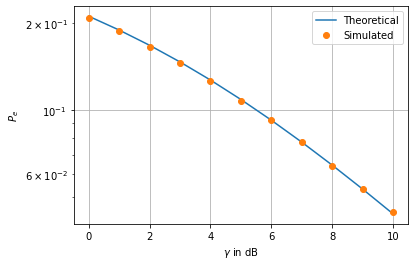
\includegraphics[scale=0.5]{images/7.4.png}
\caption{PDF}
\end{figure}
\end{enumerate}

\end{document}














